% This template was partially made with assistance from Microsoft Co-pilot

% ------------------------------------------------------------------
% CAPSTONE SOFTWARE REQUIREMENTS SPECIFICATION (SRS)

%
% This template is inspired by IEEE 29148 but simplified for use in
% a senior software engineering capstone project.
%
% The goal is not to maximize document length.
% The goal is to produce a clear, testable, and traceable set of
% requirements that can guide design, implementation, and testing.
%
% Recommended workflow:
% Stakeholder Requirements
% ->
% Use Cases
% ->
% Functional Requirements
% ->
% Acceptance Tests (will be in your VnV plan)
% ->
% Traceability Matrix (will excluded traceability for tests, that will be in the VnV plan)
%
% Students should update this document throughout the project.
% ------------------------------------------------------------------

\documentclass[12pt]{article}

\usepackage{amsmath, mathtools}
\usepackage{amsfonts}
\usepackage{amssymb}
\usepackage{graphicx}
\usepackage{colortbl}
\usepackage{xr}
\usepackage{hyperref}
\usepackage{longtable}
\usepackage{xfrac}
\usepackage{tabularx}
\usepackage{float}
\usepackage{siunitx}
\usepackage{booktabs}
\usepackage{caption}
\usepackage{pdflscape}
\usepackage{afterpage}

\usepackage[round]{natbib}

%\usepackage{refcheck}

\hypersetup{
  bookmarks=true,         % show bookmarks bar?
  colorlinks=true,       % false: boxed links; true: colored links
  linkcolor=red,          % color of internal links (change box color with linkbordercolor)
  citecolor=green,        % color of links to bibliography
  filecolor=magenta,      % color of file links
  urlcolor=cyan           % color of external links
}

\input{../Comments.text}
\input{../Common.text}

% Used so that cross-references have a meaningful prefix

\newcounter{srnum} %Stakeholder Requirement (SR) Number
\newcommand{\srthesrnum}{SR\thesrnum}
\newcommand{\srref}[1]{SR\ref{#1}}

\newcounter{ucnum} %Use Case (UC) Number
\newcommand{\uctheucnum}{UC\theucnum}
\newcommand{\ucref}[1]{UC\ref{#1}}

\newcounter{reqnum} %Functional Requirement (FR) Number
\newcommand{\rthereqnum}{FR\thereqnum}
\newcommand{\rref}[1]{FR\ref{#1}}

\newcounter{nfrnum} %Non-Functional Requirement (NFR) Number
\newcommand{\rthenfrnum}{NFR\thenfrnum}
\newcommand{\nfrref}[1]{NFR\ref{#1}}

\newcounter{lcnum} %Likely Change (LC) Number
\newcommand{\lthelcnum}{LC\thelcnum}
\newcommand{\lcref}[1]{LC\ref{#1}}

\usepackage{fullpage}

\begin{document}

  \title{Software Requirements Specification for Keystone: Capstone Project Management System}
  \author{\authname}
  \date{\today}

  \maketitle

  ~\newpage

  \pagenumbering{roman}

  \tableofcontents

  ~\newpage

  \section*{Revision History}

  \begin{tabularx}{\textwidth}{p{3cm}p{2cm}X}
\toprule {\bf Date} & {\bf Version} & {\bf Notes}\\
\midrule
Date 1 & 1.0 & Notes\\
Date 2 & 1.1 & Notes\\
\bottomrule
  \end{tabularx}

  ~\\
  \plt{All capstone SRS documents should have a reflection appendix.}

  \newpage

  \pagenumbering{arabic}

  \plt{This SRS template is based on the IEEE template, with input from co-pilot
  and S. Smith. It will get you started.  You should not modify the section
  headings, without first discussing the change with the course instructor.
  Modification means you are not following the template, which loses some of the
  advantage of a template, especially standardization.}

  \plt{Feel free to change the appearance of the report by modifying the LaTeX
  commands.}

  \plt{This template document assumes that a single program is being documented.
  If you are documenting a family of models, you should start with a commonality
  analysis.}

  \plt{The SRS is not generally written, or read, sequentially.  The SRS is a
  reference document.  It is generally read in an ad hoc order, as the need
  arises.}

  \plt{Guiding principles for the SRS document:
    \begin{itemize}
      \item Do not repeat the same information at the same abstraction level.  If
      information is repeated, the repetition should be at a different abstraction
      level.
    \end{itemize}
  }

  \plt{The template description comments should be disabled before submitting this
  document for grading.}

  \plt{You can borrow any wording from the text given in the template.  It is part
  of the template, and not considered an instance of academic integrity.  Of
  course, you need to cite the source of the template.}

  \plt{When the documentation is done, it should be possible to trace back to the
  source of every piece of information.  Some information will come from
  external sources, like terminology.}

  \plt{An SRS document should have the following qualities: unambiguous,
    consistent, complete, validatable, abstract and traceable.}

  \plt{The overall goal of the SRS is that someone can learn,
    understand and verify the captured domain knowledge.  They should not have to
    trust the authors of the SRS on any statements.  They should be able to
    independently verify/derive every statement made.}

% ==============================================================
  \section{Introduction}
% ==============================================================

  \plt{Explain what system is being specified. State purpose, users, and project goals.}

  \plt{Introduce the name of your software as \projname{}.  Using \projname{} as
  a command lets you change the name if necessary and have the change propagate to
  all documents.}

  \plt{Include a reference to the template this work is based on.  \citet{ISOIECIEEE29148_2018}
  justifies the SRS structure and \citet{ISOIECIEEE15288_2023} provides the
  broader life-cycle context that underlines modern requirements engineering
  practice.}

  This software requirements specification (SRS) document describes the system and product vision
  as well as the functional and non-functional requirements for \projname{}. The SRS is intended
  to be a reference for the development team, stakeholders, and future maintainers of the system.
  This document is constructed using the IEEE 29148 and IEEE 15288 standards
  as a guide \citep{ISOIECIEEE29148_2018, ISOIECIEEE15288_2023}.

  \subsection{Purpose}

  \plt{State the purpose of the system.}

  \plt{The purpose should be in the context of the project itself, not in the
  context of this course. Although the ``purpose'' of the document is to get a
  grade, you should not mention this.  Instead, ``fake it'' as if this is a real
  project.}

  The purpose of \projname{} is to make capstone project proposals, discovery, team formation, and
  team project approval transparent, consistent, and easy to manage for the students, supervisors, and
  course instructors involved.

  \plt{What problem does your program solve?
  The description here should be in the problem space, not the solution space.}

  Capstone project team formation, project selection, and approval currently happens across
  disconnected tools such as email, forms, and shared files, and the information in them is often
  inaccurate or out of date. As a result, students cannot tell which projects are really available,
  supervisors cannot easily see who is interested in their projects or what skills those students have,
  and instructors spend significant time coordinating the process by hand.
  See \nameref{sec:problem-statement} for a more detailed description of the problem.

  \projname{} is intended to solve these problems by giving every participant a single, trustworthy
  source of information about capstone projects, teams, and their status, from the moment a project
  is proposed until it is approved.

  \subsection{Scope}
  \plt{Briefly describe:
    \begin{itemize}
      \item Problem being solved
      \item Intended users
      \item Major functionality
      \item Expected benefits
      \item Clarifying the scope often means saying what the software doesn't do
    \end{itemize}
  }
  \plt{The scope section is relevant for understanding the boundaries of the system. It is also relevant for later determining typical values of inputs. The scope should make it clear what inputs are reasonable to expect. This is a distinction between scope and context (context is a later section).  Scope affects the inputs while context affects how the software will be used.}


\textbf{Problem being solved.} The fragmented and unreliable flow of information in capstone
  project and team selection, as described in the \nameref{sec:problem-statement} section below.

  \textbf{Intended users.} Capstone students, project supervisors (McMaster faculty and industry
  sponsors), course instructors, and teaching assistants (TAs), across the Software Engineering (SE),
  Computer Science (CS), and Mechatronics (TRON) capstone courses.

  \textbf{Major functionality.} \projname{} covers the lifecycle from project proposal to team project approval.
  Within that boundary the system:
  \begin{itemize}
    \item collects project proposals in a standardized format
    \item provides a searchable catalog of projects showing which are open, taken, or able to take
    more teams
    \item lets students create structured profiles of their skills, experience, interests, and work style
    that other students and supervisors can view, indicate whether they are looking for a team,
    and find teammates interested in the same projects
    \item suggests compatible teammates and suitable projects to students, based on their profiles and preferences
    \item lets students propose their own projects which other students and supervisors can see
    \item lets student teams express their interest to work on supervisor proposed project
    \item lets supervisors review and accept or decline interested student teams and confirm their willingness to work with a
    team;
    \item gives instructors visibility across courses into projects, teams, and their status, including
    which supervisors' projects were not selected;
    \item provides supervisors with course process, timeline, and expectation
    information, configurable by the course instructor
    \item lets students submit their team and project for instructor approval and lets teams submit later changes to
    their project information for review
    \item lets instructors approve, request changes to, or reject a team’s project submission and later changes to
    its information
  \end{itemize}

  \textbf{What \projname{} does not do.}
  \begin{itemize}
    \item It does not judge whether a project is feasible, sufficiently complex, or appropriate
    for a capstone course; this remains the responsibility of the course instructor.
    \item It does not make approval decisions. Final approval of teams and projects always rests
    with the course instructor. Courses may carry out approval inside the platform or in an external process.
    \item It does not resolve intellectual property (IP), confidentiality, or non-disclosure
    questions between students and supervisors.
    \item It does not find supervisors for student-proposed projects. Student-proposed projects are
    visible to all users of the platform, but \projname{} provides no matching or request mechanism
    for supervisors.
    \item It does not handle supervision after a project begins, such as feedback requests to
    supervisors, team performance concerns, or grading.
  \end{itemize}

  \textbf{Expected inputs.} Inputs are text-based project and profile information entered by users,
  and project status changes made by authorized users.

  \textbf{Expected benefits.} Students can compare projects reliably and avoid pursuing projects that
  are taken or misrepresented; supervisors receive better-informed applicants and fewer repeated
  emails; and instructors spend less time on repetitive coordination and gain visibility into the
  whole process.

  \subsection{Stakeholders}

    \begin{itemize}
      \item \textbf{Customer:} Course instructors for the SE, CS, and TRON capstone courses
      (Dr.~Smith, Dr.~Moradi, and Dr.~Wassyng respectively). They decide which features their course
      uses and make the final project and team approval decisions.
      \item \textbf{End Users:}
        \begin{itemize}
          \item Capstone students, who browse projects, create profiles, form teams, and apply to projects.
          \item Project supervisors, who propose projects, manage their capacity, and review and confirm
          teams. Supervisors are either McMaster faculty or industry sponsors.
          \item Course instructors and TAs, who manage users, projects, project status, and course configuration.
        \end{itemize}
      \item \textbf{Development Team:} Ayush Patel, Waqar Ul-Hassan, Ahmed Rashrash, and Andrew Habib.
    \end{itemize}

  \subsection{Definitions and Acronyms}

  \plt{This section provides the meaning of the different words and phrases used
  in the domain of the problem.}

  \begin{longtable}{p{0.25\textwidth} p{0.65\textwidth}}
    \toprule
    Term & Definition\\
    \midrule
    Capstone course & A final-year design course in which student teams spend roughly eight months
    (September to April) designing, implementing, and validating a system for a real group of
    stakeholders. In this document, the SE, CS, and TRON capstone courses.\\
    SE, CS, TRON & Software Engineering, Computer Science, and Mechatronics Engineering, the three
    programs in the Computing and Software Department whose capstone courses \projname{} supports.\\
    Course instructor & The instructor responsible for a capstone course and for approving its
    teams and projects.\\
    Supervisor & A McMaster faculty member or industry sponsor who proposes a project, or who agrees to
    advise a team on a project, and provides domain knowledge or acts as a client.\\
    Industry sponsor & A supervisor from outside McMaster, who may have no McMaster account (MacID).\\
    Project proposal & A description of a project submitted by a supervisor, or a student, for
    teams to consider.\\
    Student-proposed project & A project proposed by a student team rather than by a supervisor.\\
    Project status & The position of a project in its lifecycle, for example proposed, listed, taken,
    or approved. \\
    Supervisor capacity & The number of teams a supervisor is willing to supervise on a project.\\
    Team formation rules & Course rules on team composition: which programs may work together on
    which projects, and the minimum and maximum team size.\\
    Team project approval & The course instructor's decision to approve a team's selected project
    and membership \\
    Approval mode & How a course handles approval: in-platform, external, or integrated.\\
    Custom document & A deliverable, chosen by each team from a list, that suits the type of project
    (for example, a usability testing report).\\
    TA & Teaching assistant assigned to a capstone team after its project is approved.\\
    MacID & A McMaster University user account identifier.\\
    \bottomrule
    \caption{Definitions and Acronyms} \label{tab:DefinitionsAndAcronyms}
  \end{longtable}

  % TODO: add ``Proposal approval'' (instructor review of supervisor proposals before the list is
  % published) if Dr. Smith confirms that this is actually what he does

  \subsection{Characteristics of Intended Reader} \label{sec_IntendedReader}

  \plt{This section summarizes the skills and knowledge of the readers of the
  SRS.  It does NOT have the same purpose as the ``User Characteristics''
  section (Section~\ref{SecUserCharacteristics}).  The intended readers are the
  people that will read, review and maintain the SRS.  They are the people that
  will conceivably design the software that is intended to meet the
  requirements.  The user, on the other hand, is the person that uses the
  software that is built.  They may never read this SRS document.  Of course,
    the same person could be a ``user'' and an ``intended reader.''}

  \plt{The intended reader characteristics should be written as unambiguously and
  as specifically as possible.  Rather than say, the user should have an
  understanding of physics, say what kind of physics and at what level.  For
  instance, is high school physics adequate, or should the reader have had a
  graduate course on advanced quantum mechanics?}

  The intended reader of this SRS should have a background in software engineering,
  including knowledge of software development processes, requirements engineering,
  and system design principles. They do not have to be experts on these topics,
  but they should at least have the knowledge of a final year undergraduate student
  in software engineering. No knowledge of the capstone course process beyond the definitions
  in this section is required.

% ==============================================================
  \section{System Overview}

  This section provides general information about the system.  It identifies the
  problem, the vision, and the interfaces between the system and its environment.
  This section also describes user characteristics and lists the system
  constraints.

  \plt{The purpose of this section is to provide general information about the
  system so that the specific requirements in the later sections will be easier to
  understand. The general system description section is designed to be
  changeable independent of changes to the functional requirements documented in
  the specific system description. The general system description provides a
  context for a family of related models.  The general description can stay the
  same, while specific details are changed between family members.}

  \subsection{Problem Statement}

  \label{sec:problem-statement}

  \plt{Current situation, problem, impact, desired improvement.  You will likely borrow some text from your problem description document.}

  \textbf{Current situation.} Capstone team and project selection is spread across disconnected
  tools, including email, online forms, MS Teams, Avenue to Learn and GitLab.
  A supervisor's proposal is collected through a form and distributed to
  students as a static list. Students then form teams informally, mainly through discussion
  forums on Avenue to Learn / Teams and personal contacts, contact supervisors by email, and
  submit their chosen project and team for instructor approval through a course-specific process.
  No single place shows the state of the whole process.

  \textbf{Problems.} The following problems arise from this situation.
  \begin{itemize}
    \item \textbf{Unreliable project information.} Project descriptions vary widely in accuracy and
    detail. For example, they often do not state how much of the project already exists or what a supervisor's
    expectations are at the end. This makes projects difficult to compare and leads to mismatched expectations
    between students and supervisors.
    \item \textbf{No visibility of availability.} Students cannot see which projects are still
    available, which have been taken, or whether a supervisor is willing to take more than one team.
    After a rejection, students do not know which projects remain. Supervisors have no way to
    express how many teams they can take.
    \item \textbf{Difficulty forming teams.} Students looking for teammates currently post in a course discussion forum,
    where some describe themselves and their work style and others describe a project idea they want a team for.
    The posts are free text with no standard structure, so students cannot easily compare skills, interests,
    or work styles, or find others interested in the same project.
    \item \textbf{Student information and ideas are not visible to supervisors} Students with their own project idea
    describe it in the forum, where supervisors cannot see it. This includes supervisors who would like to
    supervise a student-proposed project. Supervisors also cannot see students’ skills, experience, or
    work style when deciding whether to work with a team. Student-proposed ideas are not tracked alongside
    supervisor-proposed projects.
    \item \textbf{Weak communication between students and supervisors.} Supervisors receive
    multiple emails from teams, including after a team has been selected, and have no structured way to learn about the
    students contacting them. Students sometimes say that a supervisor agreed to work with them even though the
    supervisor has no record of the team, so agreements must be confirmed separately.
    \item \textbf{Important information arrives too late.} Before proposing a project, supervisors receive only a
    short summary of the capstone course’s expectations and process. They learn more about its purpose, timeline,
    and expectations only after teams and projects have been settled, which leads to misunderstandings about
    what a capstone project should deliver and to many questions to the instructor.
    \item \textbf{Limited visibility for instructors.} Instructors of different capstone courses
    cannot see which projects have been selected by students in the other courses, so they cannot
    tell which proposed projects were not selected. Supervisors whose projects were not selected
    are not officially notified, leaving them in the dark and potentially discouraging them from
    proposing projects in future year.
    \item \textbf{High administrative effort for team project approval} Instructors repeat the same checks and review
    comments for many teams and students and students must fill out tedious JSON files (in SE)
    \item \textbf{Records drift after approval.} Team and project information changes after approval
    (for example, titles, supervisors, and links), but updating the official record takes effort, so
    it is often not updated and the instructor's records become out of date.
  \end{itemize}

  \textbf{Impact.} Students lose time early in a project of limited duration, teams end up
  mismatched with their projects or with each other, supervisors may become reluctant to propose
  projects in later years, and course instructors carry the administrative burden of the process.

  \textbf{Desired improvement.} All participants share a single, accurate and current source of
  information about projects, supervisors' capacity, teams, and approval status; students can find
  suitable projects and teammates; supervisors can see students’ skills and ideas and receive
  information about the course when they need it; and course instructors keep full control of
  approval decisions while spending less time on repetitive tasks.

  \subsection{Product Vision}

  \plt{A clear and concise statement of the product's purpose and goals.}

  \plt{The goal statements are functional and nonfunctional objectives that system
  under consideration should achieve. Goals provide criteria for sufficient
  completeness of a requirements specification and for requirements pertinence.
  Goals will be refined by requirements.  The goals are written abstractly, with
  a minimal amount of technical language.  They should be understandable by
  non-domain experts.}

  \plt{You will likely borrow from your goal statements in your problem
  description document.}


  \projname{} will be the central place where capstone projects are proposed, discovered, and
  matched with student teams, and where instructors can see and manage the process. Each course
  decides which features it uses and how its approval process is carried out, so the platform can
  be adopted by different courses, departments, and universities.

  The goals of \projname{} are:
  \begin{enumerate}
    \item \textbf{Reliable project information.} Every project is described in a consistent format
    that makes its objectives, required skills, current state, and expected deliverables clear.
    \item \textbf{Visibility of availability.} Users can tell which projects are open, taken, or
    able to take additional teams.
    \item \textbf{Easier team formation.} Students can describe their skills, experience, and work style
    in a structured profile, find teammates with compatible profiles and project preferences, and propose
    projects of their own for others to join.
    \item \textbf{Informed matching.} Students receive suggestions of compatible teammates and suitable projects
    based on their profiles and preferences.
    \item \textbf{Clear agreement between supervisors and teams.} A supervisor's willingness to
    work with a team is recorded in the platform and is visible to the instructor.
    \item \textbf{Informed supervisors.} Supervisors can see student-proposed projects and the skills and experience
    of the students and teams interested in their projects.
    \item \textbf{Timely process information.} Supervisors have access to information
    about the capstone course, its timeline, and its expectations, as configured by the course
    instructor.
    \item \textbf{Oversight for instructors.} Instructors can see projects, teams, supervisors,
    and their status across courses, including projects that were not selected.
    \item \textbf{Instructor-controlled approval.} Final approval decisions remain with the course
    instructor. The platform supports the approval process carried out in the course, whether that
    takes place in the platform or elsewhere.
    \item \textbf{Configurable and reusable.} Features can be turned on or off, and course-specific
    rules can be configured, so that the platform serves different courses without modification.
  \end{enumerate}

  \subsection{System Context}

  \plt{Include users, external systems, APIs, databases, and third-party services.}

  \plt{Your system context will include a figure that shows the abstract view of
  the software.  In some cases the diagram will show other external
  entities, besides the user.  For instance, when the software product is a
  library, the user will be another software program, not an actual end user.
  If there are system constraints that the software must work with external
  libraries, these libraries can also be shown on the System Context diagram.
  They should only be named with a specific library name if this is required by
  the system constraint.}

  \begin{figure}[h!]
    \begin{center}
      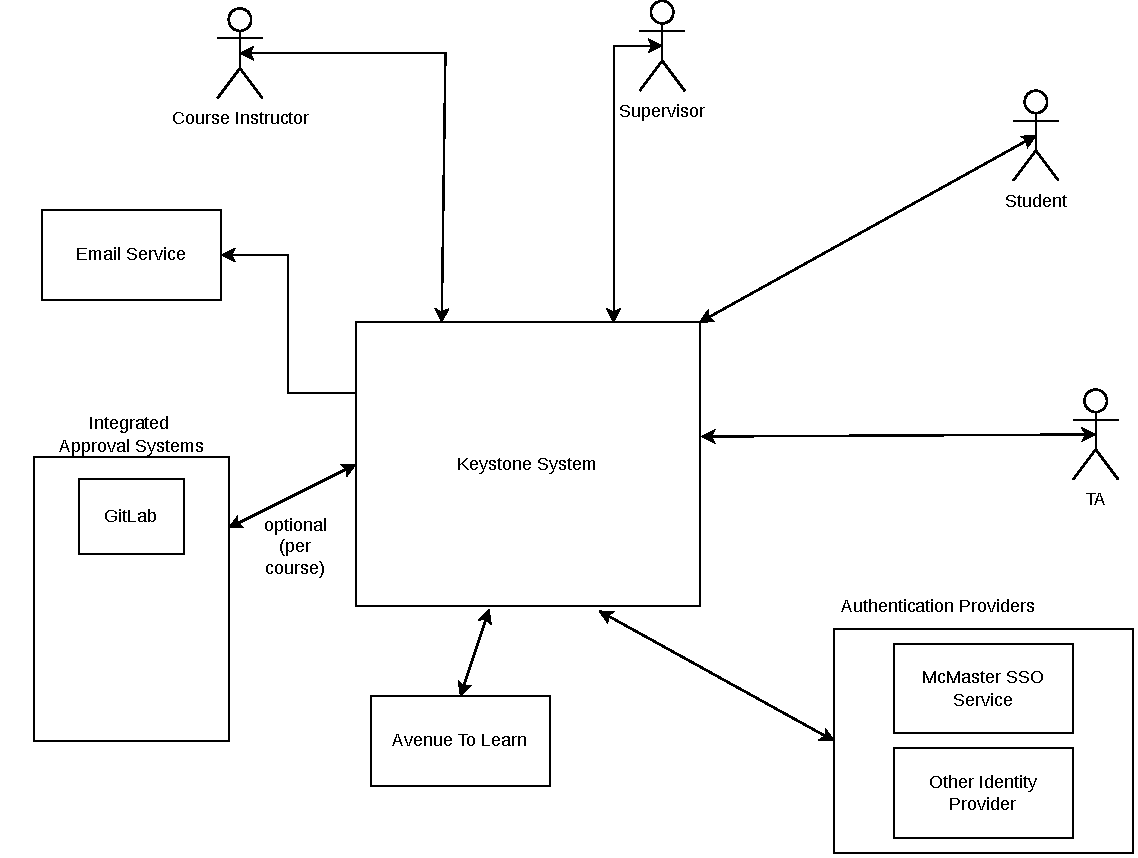
\includegraphics[width=0.6\textwidth]{SystemContextFigure}
      \caption{System Context}
      \label{Fig_SystemContext}
    \end{center}
  \end{figure}

  \plt{For each of the entities in the system context diagram its responsibilities
  should be listed.  Whenever possible the system should check for data quality,
    but for some cases the user will need to assume that responsibility.  The list
    of responsibilities should be about the inputs and outputs only, and they
    should be abstract.  Details should not be presented here.  However, the
    information should not be so abstract as to just say ``inputs'' and
    ``outputs''.  A summarizing phrase can be used to characterize the inputs.
    For instance, saying ``material properties'' provides some information, but it
    stays away from the detail of listing every required properties.}

  \begin{itemize}
    \item Student Responsibilities:
    \begin{itemize}
      \item Provide an accurate profile including skills, interests, experience, and project preferences.
      \item Express interest in projects and respond to supervisors' decisions.
      \item Provide accurate team and project information, including student-proposed projects.
    \end{itemize}
    \item Supervisor Responsibilities:
    \begin{itemize}
      \item Provide accurate, complete project proposals, including the current state of the project,
      expected outcomes, and the number of teams they are willing to supervise.
      \item Review interested teams and confirm or decline willingness to supervise them.
      \item Keep their capacity and project information current.
    \end{itemize}
    \item Course Instructor Responsibilities:
    \begin{itemize}
      \item Configure the features, rules, and approval mode that apply to their course.
      \item Make final decisions on teams and projects, including approval, requests for changes, and
      rejection.
      \item Judge project feasibility and appropriateness for the course.
      \item Provide the course process and timeline information shown to supervisors.
    \end{itemize}
    \item TA Responsibilities:
    \begin{itemize}
      \item Update project and team status as directed by instructors, in courses where approval
      takes place outside \projname{}.
      \item Assist instructors and users in keeping records accurate.
    \end{itemize}
    \item \projname{} Responsibilities:
    \begin{itemize}
      \item Check that required project, profile, and team information is present and well formed.
      \item Show current project status and availability, and supervisor capacity.
      \item Apply the team formation rules configured for each course.
      \item Restrict what each user can see and change according to their role.
      \item Record who made each change to a project or team, and when.
      \item Notify users of events that need their attention.
      \item Provide instructors with an overview of projects, teams, and their status.
      \item Suggest compatible teammates and projects based on profile data.
    \end{itemize}
  \end{itemize}

  \plt{Identify in what context the software will typically be used.  Is it for
  exploration? education? engineering work? scientific work?. Identify whether it
  will be used for mission-critical or safety-critical applications.}

  \plt{This additional context information is needed to determine how much effort
  should be devoted to the rationale section.  If the application is
  safety-critical, the bar is higher.  This is currently less structured, but
  analogous to, the idea to the Automotive Safety Integrity Levels (ASILs) that
  McSCert uses in their automotive hazard analyses.}

  \projname{} is used to coordinate an academic process. Use is concentrated around the start of
  the academic year, when projects are proposed and teams are formed, with lighter use afterwards.
  It is not mission-critical or safety-critical. A failure delays the coordination of projects and
  teams but does not cause harm. The data handled includes personal information about students, so
  privacy is the main risk to be managed, rather than safety.

  \subsection{User Characteristics} \label{SecUserCharacteristics}

  \plt{This section summarizes the knowledge/skills expected of the user.
  Measuring usability, which is often a required non-function requirement,
    requires knowledge of a typical user.  As mentioned above, the user is a
    different role from the ``intended reader,'' as given in
    Section~\ref{sec_IntendedReader}.  As in Section~\ref{sec_IntendedReader}, the
    user characteristics should be specific an unambiguous.  For instance, ``The
    end user of \projname{} should have an understanding of undergraduate Level 1
    Calculus and Physics.''}

  \begin{itemize}
    \item \textbf{Students} are final-year undergraduate students in the programs the capstone
    courses serve. They are comfortable using web applications, and many have professional
    experience from co-op placements or internships. They use \projname{} mainly at the start of the
    course, and need little training. They are motivated to find a suitable project quickly, but
    differ in whether they already have a team or a project idea.
    \item \textbf{Supervisors} are McMaster faculty or industry sponsors. They have a wide range of
    backgrounds. They may use \projname{} only a few times a year, have limited time, and may be
    unfamiliar with the capstone course, its purpose, and its timeline. Industry sponsors may have
    no McMaster account. No technical training beyond using a web application can be assumed, and
    the effort needed to propose a project must stay low enough that it does not discourage them.
    \item \textbf{Course instructors} know the course's process and rules. They configure the
    platform for their course and make approval decisions. They use it throughout the term, and need
    to configure it without developer help.
    \item \textbf{TAs} are graduate students who know the course's process. They
    help instructors with day-to-day administration and are comfortable using web applications and
    technical tools.
  \end{itemize}

  \subsection{System Constraints}

  \plt{System constraints differ from other type of requirements because they
  limit the developers' options in the system design and they identify how the
  eventual system must fit into the world. This is the only place in the SRS
  where design decisions can be specified.  That is, the quality requirement for
  abstraction is relaxed here.  However, system constraints should only be
  included if they are truly required.}

  \plt{This is where you would mention platform constrains, and licensing
  restrictions.}

  \begin{itemize}
    \item \textbf{Web-based.} \projname{} shall be accessible through current versions of common web
    browsers on desktop, tablet, and mobile devices, and shall not require specialized hardware or
    installation. An internet connection is required.
    \item \textbf{Modular features.} Each major feature shall be able to be enabled or disabled
    independently for each course, so that a course can use only the parts that fit its process.
    \item \textbf{Independent of any one approval tool.} \projname{} shall not depend on a specific
    external tool, such as the GitLab merge request process used by the Software Engineering course,
    to function. It shall support courses that carry out approval in the platform, courses that carry
    it out elsewhere, and, where an adapter exists, courses that synchronize with an external process.
    \item \textbf{Users outside the university.} \projname{} shall support users who do not have a
    McMaster account (such as industry sponsors) alongside users who do.
  \end{itemize}

% ==============================================================
  \section{Stakeholder Requirements}

  \plt{Technology-independent requirements.  These come from statements made by
  the stakeholders.  You will find these through interviews and surveys.  They are
  often expressed in natural language.  They are not necessarily testable, but
  they should be verifiable.}

  \plt{The stakeholder requirements are numbered so that you can have traceability to other parts of your document.}

  \noindent \begin{itemize}

              \item[SR\refstepcounter{srnum}\thesrnum \label{SR_Label1}] TODO

              \item[SR\refstepcounter{srnum}\thesrnum \label{SR_Label2}] TODO

              \item[SR\refstepcounter{srnum}\thesrnum \label{SR_Label3}] TODO

  \end{itemize}

  \plt{You should give your SRs meaningful labels, so that you can refer to them
  in other parts of the SRS.  The label names should be meaningful mnemonics, not
  numbers.}

% ==============================================================
  \section{User Personas}
  \plt{Create 2-5 realistic personas.
  Personas are fictional characters that represent the different user types that
  might use your software.  They are used to help understand the users'
  needs, experiences, behaviors and goals.  They are not real people, but they
  should be based on real data collected from user research.}

  \subsection{Persona 1}
  \begin{itemize}
    \item Name:
    \item Description:
    \item Goals:
    \item Frustrations:
    \item Technical Ability:
  \end{itemize}

  \subsection{Persona 2}
  \begin{itemize}
    \item Name:
    \item Description:
    \item Goals:
    \item Frustrations:
    \item Technical Ability:
  \end{itemize}

% ==============================================================
  \section{Use Cases}
  \plt{Use cases are a way to describe the interactions between users and the system.
  They are typically written in natural language and describe the steps that a
  user takes to achieve a specific goal.  Use cases can be used to identify
  functional requirements and to create test cases.}
  \plt{Typically 8-15 substantial use cases.}

  \refstepcounter{ucnum} \label{UC_Label1}
  \subsection{\ucref{UC_Label1}: Example Use Case}

  \textbf{Primary Actor}

  TODO

  \textbf{Preconditions}
  \begin{itemize}
    \item TODO
  \end{itemize}

  \textbf{Main Success Scenario}
  \begin{enumerate}
    \item TODO
    \item TODO
    \item TODO
  \end{enumerate}

  \textbf{Alternative Flows}
  \begin{itemize}
    \item TODO
  \end{itemize}

  \textbf{Postconditions}
  \begin{itemize}
    \item TODO
  \end{itemize}

% ==============================================================
  \section{Functional Requirements}
  \plt{Functional requirements describe what the system should do.  They are typically
  expressed as a set of conditions or capabilities that the system must have.  These
  requirements are usually derived from the stakeholder requirements and use cases.}

  \plt{Use SHALL statements. Requirements must be atomic, testable, and traceable.}

  \noindent \begin{itemize}

              \item[FR\refstepcounter{reqnum}\thereqnum \label{FR_Label1}:] The system shall ...

              \item[FR\refstepcounter{reqnum}\thereqnum \label{FR_Label2}:] The system shall ...

              \item[FR\refstepcounter{reqnum}\thereqnum \label{FR_Label3}:] The system shall ...

  \end{itemize}

  \plt{The requirements are given labels so that they can be referenced in other
  parts of the SRS.  The label names should be meaningful mnemonics, not numbers.}

% ==============================================================
  \section{Data Requirements}

  \plt{The Data Requirements section describes what information the system must manage.
  It includes the major data entities, their attributes, and the relationships
  between them.  It also includes a data dictionary that defines the meaning of
  each attribute.}

  \subsection{Major Data Entities}

  \plt{What information must exist for the system to accomplish its goals?}

  \plt{For each entity, provide a short explanation.}

  \begin{itemize}
    \item User
    \item Song
    \item Session
    \item Report
  \end{itemize}

  \subsection{Data Dictionary}

  \plt{For each entity, define all important attributes.}

  \begin{longtable}{p{0.20\textwidth} p{0.20\textwidth} p{0.45\textwidth}}
    \toprule
    Attribute & Type & Description\\
    \midrule
    user\_id & UUID & Unique identifier\\
    email & String & User email address\\
    \bottomrule
    \caption{Data Dictionary} \label{tab:DataDictionary}
  \end{longtable}

  \subsection{Privacy and Data Retention}

  \plt{Discuss storage, retention, deletion, privacy controls,
    consent, encryption, and compliance requirements.}

  TODO

% ==============================================================
  \section{Non-Functional Requirements}

  \plt{You may have to add other NFRs.}

  \plt{List your nonfunctional requirements.  You may consider using a fit
  criterion to make them verifiable.}

  \plt{The goal is for the nonfunctional requirements to be unambiguous, abstract
  and verifiable.  This isn't easy to show succinctly, so a good strategy may be
  to give a ``high level'' view of the requirement, but allow for the details to
  be covered in the Verification and Validation document.}

  \plt{An absolute requirement on a quality of the system is rarely needed.  For
  instance, an accuracy of 0.0101 \% is likely fine, even if the requirement is
  for 0.01 \% accuracy.  Therefore, the emphasis will often be more on
  describing now well the quality is achieved, through experimentation, and
  possibly theory, rather than meeting some bar that was defined a priori.}

  \plt{You do not need an entry for correctness in your NFRs.  The purpose of the
  SRS is to record the requirements that need to be satisfied for correctness.
  Any statement of correctness would just be redundant. Rather than discuss
  correctness, you can characterize how far away from the correct (true)
    solution you are allowed to be.  This is discussed under accuracy.}

  \noindent \begin{itemize}

              \item[NFR\refstepcounter{nfrnum}\thenfrnum \label{NFR_Accuracy}:]
              \textbf{Accuracy} \plt{Characterize the accuracy by giving the context/use for
              the software.  Maybe something like, ``The accuracy of the computed
              solutions should meet the level needed for $<$engineering or scientific
              application$>$.  The level of accuracy achieved by \projname{} shall be
              described following the procedure given in Section~X of the Verification and
              Validation Plan.''  If you do this provide a link to the VnV plan.}

              \item[NFR\refstepcounter{nfrnum}\thenfrnum \label{NFR_Usability}:] \textbf{Usability}
              \plt{Characterize the usability by giving the context/use for the software.
              You should likely reference the user characteristics section.  The level of
              usability achieved by the software shall be described following the
              procedure given in Section~X of the Verification and Validation Plan.  Include a link to the VnV plan.}

              \item[NFR\refstepcounter{nfrnum}\thenfrnum \label{NFR_Maintainability}:]
              \textbf{Maintainability} \plt{The effort required to make any of the likely
              changes listed for \projname{} should be less than FRACTION of the original
              development time.  FRACTION is then a symbolic constant that can be defined
              at the end of the report.}

              \item[NFR\refstepcounter{nfrnum}\thenfrnum \label{NFR_Portability}:]
              \textbf{Portability} \plt{This NFR is easier to write than the others.  The
              systems that \projname{} should run on should be listed here.  When possible
              the specific versions of the potential operating environments should be
              given.  To make the NFR verifiable a statement could be made that the tests
              from a given section of the VnV plan can be successfully run on all of the
              possible operating environments.}

              \item Other NFRs that might be discussed include verifiability,
              understandability, reusability, performance, reliability and availability, security, and accessibility.  You may have to add other NFRs.

  \end{itemize}

% ==============================================================
  \section{AI and Machine Learning Requirements}

  \plt{Refer to
  \href{https://gitlab.cas.mcmaster.ca/courses/capstone/-/blob/main/Lectures/Lxx_DrMosserGuestLecture/2026_09_Capstone.pdf?ref_type=heads}{Dr.
  Mosser's guest lecture} on AI requirements.}

  \plt{Include only when applicable.}

  \subsection{Model Inputs}

  TODO

  \subsection{Model Outputs}

  TODO

  \subsection{Evaluation Metrics}

  \plt{Accuracy, Precision, Recall, F1, BLEU, WER, etc.}

  TODO

  \subsection{Known Limitations}

  \plt{Explicitly document expected failure modes.}

  TODO

% ==============================================================
  \section{Requirements Traceability Matrices}

  \plt{The Requirements Traceability Matrix (RTM) is a table that shows the
  relationship between different types of requirements. It is used to ensure that
  all requirements are traceable and that no requirements are missed. The typical
  flow is: Stakeholder Need -> Use Case -> Requirement}

  \plt{There is also a traceability matrix between functional and nonfunctional
  requirements. The purpose of some FRs is to satisfy NFRs.  Therefore, it is
  important to show the relationship between the two.}

  \plt{Further traceability to test cases and modules will be given in other
  documents.}

  \begin{longtable}{p{0.15\textwidth} p{0.15\textwidth} p{0.20\textwidth} p{0.20\textwidth}}

    \toprule
    Stakeholder Req & Use Case & Functional Req \\
    \midrule
    \srref{SR_Label1} & \ucref{UC_Label1} & \rref{FR_Label1} \\
    \bottomrule

    \caption{Traceability Between Stakeholder Requirements, Use Cases, and
    Functional Requirements} \label{tab:SR2UC2FRtm}
  \end{longtable}

  \begin{longtable}{p{0.20\textwidth} p{0.20\textwidth}}

    \toprule
    Functional Req & Nonfunctional Req \\
    \midrule
    \rref{FR_Label1} & \nfrref{NFR_Accuracy} \\
    \bottomrule
    \caption{Traceability Between Functional and Nonfunctional Requirements}
    \label{tab:FR2Rtm}

  \end{longtable}

% ==============================================================

  \section{Rationale}

  \plt{Provide a rationale for the decisions made in the documentation.  Rationale
  should be provided for scope decisions, functional requirements, nonfunctioanl
  requirements, data requirements, and AI requirements.  You don't need a
  rationale for everything, ust the major decisions that are not obvious.  You
  should have traceability to the entities in the document that you are
  referencing.}

  \section{Likely Changes}

  \noindent \begin{itemize}

              \item[LC\refstepcounter{lcnum}\thelcnum\label{LC_meaningfulLabel}:] \plt{Give
              the likely changes, with traceability to the entity that is likely to change.}

  \end{itemize}

  \section{Unlikely Changes}

  \noindent \begin{itemize}

              \item[LC\refstepcounter{lcnum}\thelcnum\label{LC_meaningfulLabel}:] \plt{Give
              the unlikely changes.  The design can assume that the changes listed will
              not occur.}

  \end{itemize}

  \newpage{}

  \section{Appendices}

  \subsection{Appendix A: Additional Materials}

  TODO

  \subsection{Appendix B: Development Plan}

  \plt{This section is optional.  It is used to explain the plan for developing
  the software.  In particular, this section gives a list of the order in which
  the requirements will be implemented.  In the context of a course  this is
  where you can indicate which requirements will be implemented as part of the
  course, and which will be ``faked'' as future work.  This section can be
  organized as a prioritized list of requirements, or it could show the
  requirements that will be implemented for ``phase 1'', ``phase 2'', etc.}

  \subsection{Appendix C: Values of Auxiliary Constants}

  \plt{Show the values of the symbolic parameters introduced in the report.}

  \plt{The definition of the requirements will likely call for SYMBOLIC\_CONSTANTS.
  Their values are defined in this section for easy maintenance.}

  \plt{The value of FRACTION, for the Maintainability NFR would be given here.}

  TODO

  \subsection{Appendix D: Generative AI Disclosure}

  \plt{Provide full transparency on how generative AI was used in the creation of
  this document.  This includes any text, figures, or tables that were generated
  by AI.  If any skills were created for AI agents to review the documentation,
    those should be disclosed here.}

  \subsection{Appendix E: Reflection}

  \plt{This isn't part of the SRS, but it is part of the course.}

  The information in this section will be used to evaluate the team members on the
  graduate attribute of Lifelong Learning.

  \input{../Reflection.text}

  \input{../SRS_Reflection.text}

  \newpage

  \bibliographystyle {plainnat}
  \bibliography {../../refs/References}

  \newpage


\end{document}